\documentclass[1p]{elsarticle_modified}
%\bibliographystyle{elsarticle-num}

%\usepackage[colorlinks]{hyperref}
%\usepackage{abbrmath_seonhwa} %\Abb, \Ascr, \Acal ,\Abf, \Afrak
\usepackage{amsfonts}
\usepackage{amssymb}
\usepackage{amsmath}
\usepackage{amsthm}
\usepackage{scalefnt}
\usepackage{amsbsy}
\usepackage{kotex}
\usepackage{caption}
\usepackage{subfig}
\usepackage{color}
\usepackage{graphicx}
\usepackage{xcolor} %% white, black, red, green, blue, cyan, magenta, yellow
\usepackage{float}
\usepackage{setspace}
\usepackage{hyperref}

\usepackage{tikz}
\usetikzlibrary{arrows}

\usepackage{multirow}
\usepackage{array} % fixed length table
\usepackage{hhline}

%%%%%%%%%%%%%%%%%%%%%
\makeatletter
\renewcommand*\env@matrix[1][\arraystretch]{%
	\edef\arraystretch{#1}%
	\hskip -\arraycolsep
	\let\@ifnextchar\new@ifnextchar
	\array{*\c@MaxMatrixCols c}}
\makeatother %https://tex.stackexchange.com/questions/14071/how-can-i-increase-the-line-spacing-in-a-matrix
%%%%%%%%%%%%%%%

\usepackage[normalem]{ulem}

\newcommand{\msout}[1]{\ifmmode\text{\sout{\ensuremath{#1}}}\else\sout{#1}\fi}
%SOURCE: \msout is \stkout macro in https://tex.stackexchange.com/questions/20609/strikeout-in-math-mode

\newcommand{\cancel}[1]{
	\ifmmode
	{\color{red}\msout{#1}}
	\else
	{\color{red}\sout{#1}}
	\fi
}

\newcommand{\add}[1]{
	{\color{blue}\uwave{#1}}
}

\newcommand{\replace}[2]{
	\ifmmode
	{\color{red}\msout{#1}}{\color{blue}\uwave{#2}}
	\else
	{\color{red}\sout{#1}}{\color{blue}\uwave{#2}}
	\fi
}

\newcommand{\Sol}{\mathcal{S}} %segment
\newcommand{\D}{D} %diagram
\newcommand{\A}{\mathcal{A}} %arc


%%%%%%%%%%%%%%%%%%%%%%%%%%%%%5 test

\def\sl{\operatorname{\textup{SL}}(2,\Cbb)}
\def\psl{\operatorname{\textup{PSL}}(2,\Cbb)}
\def\quan{\mkern 1mu \triangleright \mkern 1mu}

\theoremstyle{definition}
\newtheorem{thm}{Theorem}[section]
\newtheorem{prop}[thm]{Proposition}
\newtheorem{lem}[thm]{Lemma}
\newtheorem{ques}[thm]{Question}
\newtheorem{cor}[thm]{Corollary}
\newtheorem{defn}[thm]{Definition}
\newtheorem{exam}[thm]{Example}
\newtheorem{rmk}[thm]{Remark}
\newtheorem{alg}[thm]{Algorithm}

\newcommand{\I}{\sqrt{-1}}
\begin{document}

%\begin{frontmatter}
%
%\title{Boundary parabolic representations of knots up to 8 crossings}
%
%%% Group authors per affiliation:
%\author{Yunhi Cho} 
%\address{Department of Mathematics, University of Seoul, Seoul, Korea}
%\ead{yhcho@uos.ac.kr}
%
%
%\author{Seonhwa Kim} %\fnref{s_kim}}
%\address{Center for Geometry and Physics, Institute for Basic Science, Pohang, 37673, Korea}
%\ead{ryeona17@ibs.re.kr}
%
%\author{Hyuk Kim}
%\address{Department of Mathematical Sciences, Seoul National University, Seoul 08826, Korea}
%\ead{hyukkim@snu.ac.kr}
%
%\author{Seokbeom Yoon}
%\address{Department of Mathematical Sciences, Seoul National University, Seoul, 08826,  Korea}
%\ead{sbyoon15@snu.ac.kr}
%
%\begin{abstract}
%We find all boundary parabolic representation of knots up to 8 crossings.
%
%\end{abstract}
%\begin{keyword}
%    \MSC[2010] 57M25 
%\end{keyword}
%
%\end{frontmatter}

%\linenumbers
%\tableofcontents
%
\newcommand\colored[1]{\textcolor{white}{\rule[-0.35ex]{0.8em}{1.4ex}}\kern-0.8em\color{red} #1}%
%\newcommand\colored[1]{\textcolor{white}{ #1}\kern-2.17ex	\textcolor{white}{ #1}\kern-1.81ex	\textcolor{white}{ #1}\kern-2.15ex\color{red}#1	}

{\Large $\underline{12n_{0783}~(K12n_{0783})}$}

\setlength{\tabcolsep}{10pt}
\renewcommand{\arraystretch}{1.6}
\vspace{1cm}\begin{tabular}{m{100pt}>{\centering\arraybackslash}m{274pt}}
\multirow{5}{120pt}{
	\centering
	\includegraphics[width=112pt]{../../../GIT/diagram.site/Diagrams/png/2872_12n_0783.png}\\
\ \ \ A knot diagram\footnotemark}&
\allowdisplaybreaks
\textbf{Linearized knot diagam} \\
\cline{2-2}
 &
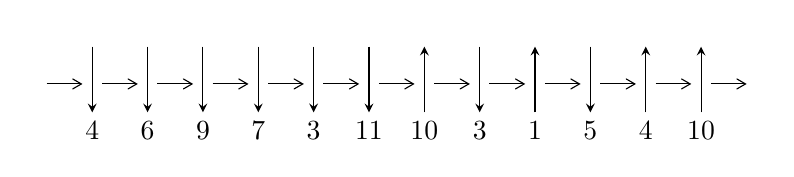
\begin{tikzpicture}[x=20pt, y=17pt]
	% nodes
	\node (C0) at (0, 0) {};
	\node (C1) at (1, 0) {};
	\node (C1U) at (1, +1) {};
	\node (C1D) at (1, -1) {4};

	\node (C2) at (2, 0) {};
	\node (C2U) at (2, +1) {};
	\node (C2D) at (2, -1) {6};

	\node (C3) at (3, 0) {};
	\node (C3U) at (3, +1) {};
	\node (C3D) at (3, -1) {9};

	\node (C4) at (4, 0) {};
	\node (C4U) at (4, +1) {};
	\node (C4D) at (4, -1) {7};

	\node (C5) at (5, 0) {};
	\node (C5U) at (5, +1) {};
	\node (C5D) at (5, -1) {3};

	\node (C6) at (6, 0) {};
	\node (C6U) at (6, +1) {};
	\node (C6D) at (6, -1) {11};

	\node (C7) at (7, 0) {};
	\node (C7U) at (7, +1) {};
	\node (C7D) at (7, -1) {10};

	\node (C8) at (8, 0) {};
	\node (C8U) at (8, +1) {};
	\node (C8D) at (8, -1) {3};

	\node (C9) at (9, 0) {};
	\node (C9U) at (9, +1) {};
	\node (C9D) at (9, -1) {1};

	\node (C10) at (10, 0) {};
	\node (C10U) at (10, +1) {};
	\node (C10D) at (10, -1) {5};

	\node (C11) at (11, 0) {};
	\node (C11U) at (11, +1) {};
	\node (C11D) at (11, -1) {4};

	\node (C12) at (12, 0) {};
	\node (C12U) at (12, +1) {};
	\node (C12D) at (12, -1) {10};
	\node (C13) at (13, 0) {};

	% arrows
	\draw[->,>={angle 60}]
	(C0) edge (C1) (C1) edge (C2) (C2) edge (C3) (C3) edge (C4) (C4) edge (C5) (C5) edge (C6) (C6) edge (C7) (C7) edge (C8) (C8) edge (C9) (C9) edge (C10) (C10) edge (C11) (C11) edge (C12) (C12) edge (C13) ;	\draw[->,>=stealth]
	(C1U) edge (C1D) (C2U) edge (C2D) (C3U) edge (C3D) (C4U) edge (C4D) (C5U) edge (C5D) (C6U) edge (C6D) (C7D) edge (C7U) (C8U) edge (C8D) (C9D) edge (C9U) (C10U) edge (C10D) (C11D) edge (C11U) (C12D) edge (C12U) ;
	\end{tikzpicture} \\
\hhline{~~} \\& 
\textbf{Solving Sequence} \\ \cline{2-2} 
 &
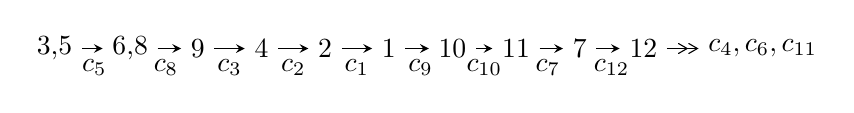
\begin{tikzpicture}[x=23pt, y=7pt]
	% node
	\node (A0) at (-1/8, 0) {3,5};
	\node (A1) at (17/16, 0) {6,8};
	\node (A2) at (17/8, 0) {9};
	\node (A3) at (25/8, 0) {4};
	\node (A4) at (33/8, 0) {2};
	\node (A5) at (41/8, 0) {1};
	\node (A6) at (49/8, 0) {10};
	\node (A7) at (57/8, 0) {11};
	\node (A8) at (65/8, 0) {7};
	\node (A9) at (73/8, 0) {12};
	\node (C1) at (1/2, -1) {$c_{5}$};
	\node (C2) at (13/8, -1) {$c_{8}$};
	\node (C3) at (21/8, -1) {$c_{3}$};
	\node (C4) at (29/8, -1) {$c_{2}$};
	\node (C5) at (37/8, -1) {$c_{1}$};
	\node (C6) at (45/8, -1) {$c_{9}$};
	\node (C7) at (53/8, -1) {$c_{10}$};
	\node (C8) at (61/8, -1) {$c_{7}$};
	\node (C9) at (69/8, -1) {$c_{12}$};
	\node (A10) at (11, 0) {$c_{4},c_{6},c_{11}$};

	% edge
	\draw[->,>=stealth]	
	(A0) edge (A1) (A1) edge (A2) (A2) edge (A3) (A3) edge (A4) (A4) edge (A5) (A5) edge (A6) (A6) edge (A7) (A7) edge (A8) (A8) edge (A9) ;
	\draw[->>,>={angle 60}]	
	(A9) edge (A10);
\end{tikzpicture} \\ 

\end{tabular} \\

\footnotetext{
The image of knot diagram is generated by the software ``\textbf{Draw programme}" developed by Andrew Bartholomew(\url{http://www.layer8.co.uk/maths/draw/index.htm\#Running-draw}), where we modified some parts for our purpose(\url{https://github.com/CATsTAILs/LinksPainter}).
}\phantom \\ \newline 
\centering \textbf{Ideals for irreducible components\footnotemark of $X_{\text{par}}$} 
 
\begin{align*}
I^u_{1}&=\langle 
-5.05060\times10^{389} u^{96}+5.72708\times10^{389} u^{95}+\cdots+2.60152\times10^{390} b+2.75118\times10^{390},\\
\phantom{I^u_{1}}&\phantom{= \langle  }-2.62698\times10^{389} u^{96}+8.51804\times10^{389} u^{95}+\cdots+2.60152\times10^{390} a-6.09559\times10^{391},\\
\phantom{I^u_{1}}&\phantom{= \langle  }u^{97}- u^{96}+\cdots-26 u-1\rangle \\
I^u_{2}&=\langle 
2.13340\times10^{23} u^{33}+3.36277\times10^{23} u^{32}+\cdots+5.15575\times10^{22} b-2.19695\times10^{23},\\
\phantom{I^u_{2}}&\phantom{= \langle  }6.92894\times10^{22} u^{33}+2.64178\times10^{22} u^{32}+\cdots+5.15575\times10^{22} a+3.17866\times10^{22},\;u^{34}+2 u^{33}+\cdots+2 u+1\rangle \\
\\
\end{align*}
\raggedright * 2 irreducible components of $\dim_{\mathbb{C}}=0$, with total 131 representations.\\
\footnotetext{All coefficients of polynomials are rational numbers. But the coefficients are sometimes approximated in decimal forms when there is not enough margin.}
\newpage
\renewcommand{\arraystretch}{1}
\centering \section*{I. $I^u_{1}= \langle -5.05\times10^{389} u^{96}+5.73\times10^{389} u^{95}+\cdots+2.60\times10^{390} b+2.75\times10^{390},\;-2.63\times10^{389} u^{96}+8.52\times10^{389} u^{95}+\cdots+2.60\times10^{390} a-6.10\times10^{391},\;u^{97}- u^{96}+\cdots-26 u-1 \rangle$}
\flushleft \textbf{(i) Arc colorings}\\
\begin{tabular}{m{7pt} m{180pt} m{7pt} m{180pt} }
\flushright $a_{3}=$&$\begin{pmatrix}0\\u\end{pmatrix}$ \\
\flushright $a_{5}=$&$\begin{pmatrix}1\\0\end{pmatrix}$ \\
\flushright $a_{6}=$&$\begin{pmatrix}1\\u^2\end{pmatrix}$ \\
\flushright $a_{8}=$&$\begin{pmatrix}0.100978 u^{96}-0.327425 u^{95}+\cdots+391.203 u+23.4308\\0.194140 u^{96}-0.220143 u^{95}+\cdots-21.0064 u-1.05753\end{pmatrix}$ \\
\flushright $a_{9}=$&$\begin{pmatrix}0.100978 u^{96}-0.327425 u^{95}+\cdots+391.203 u+23.4308\\0.220457 u^{96}-0.252020 u^{95}+\cdots-26.7930 u-1.28397\end{pmatrix}$ \\
\flushright $a_{4}=$&$\begin{pmatrix}1.23839 u^{96}-1.73803 u^{95}+\cdots+326.757 u+15.7854\\0.170008 u^{96}-0.191437 u^{95}+\cdots-15.7017 u-0.857083\end{pmatrix}$ \\
\flushright $a_{2}=$&$\begin{pmatrix}u\\u^3+u\end{pmatrix}$ \\
\flushright $a_{1}=$&$\begin{pmatrix}-3.70848 u^{96}+4.83210 u^{95}+\cdots+72.9539 u+16.7184\\0.211595 u^{96}-0.250722 u^{95}+\cdots-36.1278 u-1.45422\end{pmatrix}$ \\
\flushright $a_{10}=$&$\begin{pmatrix}-3.59279 u^{96}+4.62876 u^{95}+\cdots-240.869 u-6.99467\\-0.0810977 u^{96}+0.0659827 u^{95}+\cdots+3.16747 u+0.177008\end{pmatrix}$ \\
\flushright $a_{11}=$&$\begin{pmatrix}-3.51169 u^{96}+4.56278 u^{95}+\cdots-244.037 u-7.17168\\-0.0810977 u^{96}+0.0659827 u^{95}+\cdots+3.16747 u+0.177008\end{pmatrix}$ \\
\flushright $a_{7}=$&$\begin{pmatrix}-8.70315 u^{96}+9.85411 u^{95}+\cdots+771.754 u+31.4956\\0.318091 u^{96}-0.370413 u^{95}+\cdots-44.5790 u-2.59273\end{pmatrix}$ \\
\flushright $a_{12}=$&$\begin{pmatrix}-7.27267 u^{96}+9.07460 u^{95}+\cdots-250.054 u-15.9505\\-0.429364 u^{96}+0.436517 u^{95}+\cdots+57.8522 u+2.72828\end{pmatrix}$\\&\end{tabular}
\flushleft \textbf{(ii) Obstruction class $= -1$}\\~\\
\flushleft \textbf{(iii) Cusp Shapes $= 4.81068 u^{96}-5.73756 u^{95}+\cdots-506.753 u-29.0779$}\\~\\
\newpage\renewcommand{\arraystretch}{1}
\flushleft \textbf{(iv) u-Polynomials at the component}\newline \\
\begin{tabular}{m{50pt}|m{274pt}}
Crossings & \hspace{64pt}u-Polynomials at each crossing \\
\hline $$\begin{aligned}c_{1}\end{aligned}$$&$\begin{aligned}
&u^{97}-11 u^{96}+\cdots-374950992 u+77123381
\end{aligned}$\\
\hline $$\begin{aligned}c_{2},c_{5}\end{aligned}$$&$\begin{aligned}
&u^{97}+u^{96}+\cdots-26 u+1
\end{aligned}$\\
\hline $$\begin{aligned}c_{3},c_{8}\end{aligned}$$&$\begin{aligned}
&u^{97}- u^{96}+\cdots-1679 u+193
\end{aligned}$\\
\hline $$\begin{aligned}c_{4}\end{aligned}$$&$\begin{aligned}
&u^{97}-5 u^{96}+\cdots+2 u+1
\end{aligned}$\\
\hline $$\begin{aligned}c_{6}\end{aligned}$$&$\begin{aligned}
&u^{97}+u^{96}+\cdots-51516 u+41391
\end{aligned}$\\
\hline $$\begin{aligned}c_{7}\end{aligned}$$&$\begin{aligned}
&u^{97}+5 u^{96}+\cdots-340064 u+80363
\end{aligned}$\\
\hline $$\begin{aligned}c_{9},c_{12}\end{aligned}$$&$\begin{aligned}
&u^{97}-6 u^{96}+\cdots+369 u+77
\end{aligned}$\\
\hline $$\begin{aligned}c_{10}\end{aligned}$$&$\begin{aligned}
&u^{97}- u^{96}+\cdots-334 u+5
\end{aligned}$\\
\hline $$\begin{aligned}c_{11}\end{aligned}$$&$\begin{aligned}
&u^{97}-3 u^{96}+\cdots+1176280393 u+231783103
\end{aligned}$\\
\hline
\end{tabular}\\~\\
\newpage\renewcommand{\arraystretch}{1}
\flushleft \textbf{(v) Riley Polynomials at the component}\newline \\
\begin{tabular}{m{50pt}|m{274pt}}
Crossings & \hspace{64pt}Riley Polynomials at each crossing \\
\hline $$\begin{aligned}c_{1}\end{aligned}$$&$\begin{aligned}
&y^{97}+19 y^{96}+\cdots-39629618873565244 y-5948015896871161
\end{aligned}$\\
\hline $$\begin{aligned}c_{2},c_{5}\end{aligned}$$&$\begin{aligned}
&y^{97}+71 y^{96}+\cdots-140 y-1
\end{aligned}$\\
\hline $$\begin{aligned}c_{3},c_{8}\end{aligned}$$&$\begin{aligned}
&y^{97}-33 y^{96}+\cdots+1583455 y-37249
\end{aligned}$\\
\hline $$\begin{aligned}c_{4}\end{aligned}$$&$\begin{aligned}
&y^{97}-3 y^{96}+\cdots-282 y-1
\end{aligned}$\\
\hline $$\begin{aligned}c_{6}\end{aligned}$$&$\begin{aligned}
&y^{97}+19 y^{96}+\cdots-63141732036 y-1713214881
\end{aligned}$\\
\hline $$\begin{aligned}c_{7}\end{aligned}$$&$\begin{aligned}
&y^{97}-45 y^{96}+\cdots+204622080600 y-6458211769
\end{aligned}$\\
\hline $$\begin{aligned}c_{9},c_{12}\end{aligned}$$&$\begin{aligned}
&y^{97}+28 y^{96}+\cdots+6185 y-5929
\end{aligned}$\\
\hline $$\begin{aligned}c_{10}\end{aligned}$$&$\begin{aligned}
&y^{97}+21 y^{96}+\cdots-93964 y-25
\end{aligned}$\\
\hline $$\begin{aligned}c_{11}\end{aligned}$$&$\begin{aligned}
&y^{97}-53 y^{96}+\cdots+630230524010700897 y-53723406836308609
\end{aligned}$\\
\hline
\end{tabular}\\~\\
\newpage\flushleft \textbf{(vi) Complex Volumes and Cusp Shapes}
$$\begin{array}{c|c|c}  
\text{Solutions to }I^u_{1}& \I (\text{vol} + \sqrt{-1}CS) & \text{Cusp shape}\\
 \hline 
\begin{aligned}
u &= -0.760246 + 0.714813 I \\
a &= -0.193608 - 0.566947 I \\
b &= -0.731753 + 0.243850 I\end{aligned}
 & -3.28969 - 1.97027 I & \phantom{-0.000000 } 0 \\ \hline\begin{aligned}
u &= -0.760246 - 0.714813 I \\
a &= -0.193608 + 0.566947 I \\
b &= -0.731753 - 0.243850 I\end{aligned}
 & -3.28969 + 1.97027 I & \phantom{-0.000000 } 0 \\ \hline\begin{aligned}
u &= -0.657532 + 0.609454 I \\
a &= \phantom{-}0.726346 + 0.262206 I \\
b &= \phantom{-}0.083124 - 0.807986 I\end{aligned}
 & \phantom{-}0.47950 + 4.79117 I & \phantom{-0.000000 } 0 \\ \hline\begin{aligned}
u &= -0.657532 - 0.609454 I \\
a &= \phantom{-}0.726346 - 0.262206 I \\
b &= \phantom{-}0.083124 + 0.807986 I\end{aligned}
 & \phantom{-}0.47950 - 4.79117 I & \phantom{-0.000000 } 0 \\ \hline\begin{aligned}
u &= \phantom{-}0.685034 + 0.878100 I \\
a &= -0.675640 + 0.593394 I \\
b &= -1.044380 + 0.432774 I\end{aligned}
 & -1.28499 - 4.64287 I & \phantom{-0.000000 } 0 \\ \hline\begin{aligned}
u &= \phantom{-}0.685034 - 0.878100 I \\
a &= -0.675640 - 0.593394 I \\
b &= -1.044380 - 0.432774 I\end{aligned}
 & -1.28499 + 4.64287 I & \phantom{-0.000000 } 0 \\ \hline\begin{aligned}
u &= \phantom{-}0.075161 + 1.114100 I \\
a &= \phantom{-}0.416477 - 1.110930 I \\
b &= \phantom{-}0.878909 + 0.357543 I\end{aligned}
 & -1.86695 + 1.01835 I & \phantom{-0.000000 } 0 \\ \hline\begin{aligned}
u &= \phantom{-}0.075161 - 1.114100 I \\
a &= \phantom{-}0.416477 + 1.110930 I \\
b &= \phantom{-}0.878909 - 0.357543 I\end{aligned}
 & -1.86695 - 1.01835 I & \phantom{-0.000000 } 0 \\ \hline\begin{aligned}
u &= \phantom{-}0.016883 + 0.882984 I \\
a &= -0.123207 + 0.633830 I \\
b &= -0.588620 - 0.214403 I\end{aligned}
 & \phantom{-}2.45092 - 1.33246 I & \phantom{-0.000000 } 0 \\ \hline\begin{aligned}
u &= \phantom{-}0.016883 - 0.882984 I \\
a &= -0.123207 - 0.633830 I \\
b &= -0.588620 + 0.214403 I\end{aligned}
 & \phantom{-}2.45092 + 1.33246 I & \phantom{-0.000000 } 0\\
 \hline 
 \end{array}$$\newpage$$\begin{array}{c|c|c}  
\text{Solutions to }I^u_{1}& \I (\text{vol} + \sqrt{-1}CS) & \text{Cusp shape}\\
 \hline 
\begin{aligned}
u &= -0.375100 + 1.079430 I \\
a &= -1.249720 + 0.232941 I \\
b &= -1.68979 - 0.00461 I\end{aligned}
 & \phantom{-}4.32226 + 1.56783 I & \phantom{-0.000000 } 0 \\ \hline\begin{aligned}
u &= -0.375100 - 1.079430 I \\
a &= -1.249720 - 0.232941 I \\
b &= -1.68979 + 0.00461 I\end{aligned}
 & \phantom{-}4.32226 - 1.56783 I & \phantom{-0.000000 } 0 \\ \hline\begin{aligned}
u &= -0.698909 + 0.927947 I \\
a &= \phantom{-}0.674038 + 0.385290 I \\
b &= \phantom{-}1.170460 - 0.394638 I\end{aligned}
 & -2.66934 + 7.52224 I & \phantom{-0.000000 } 0 \\ \hline\begin{aligned}
u &= -0.698909 - 0.927947 I \\
a &= \phantom{-}0.674038 - 0.385290 I \\
b &= \phantom{-}1.170460 + 0.394638 I\end{aligned}
 & -2.66934 - 7.52224 I & \phantom{-0.000000 } 0 \\ \hline\begin{aligned}
u &= -1.192060 + 0.013477 I \\
a &= -0.650672 + 0.794722 I \\
b &= -0.665573 - 0.387174 I\end{aligned}
 & \phantom{-}3.36728 + 4.65708 I & \phantom{-0.000000 } 0 \\ \hline\begin{aligned}
u &= -1.192060 - 0.013477 I \\
a &= -0.650672 - 0.794722 I \\
b &= -0.665573 + 0.387174 I\end{aligned}
 & \phantom{-}3.36728 - 4.65708 I & \phantom{-0.000000 } 0 \\ \hline\begin{aligned}
u &= -0.143111 + 1.228920 I \\
a &= -1.059730 - 0.651904 I \\
b &= -2.01954 - 0.49278 I\end{aligned}
 & \phantom{-}5.83853 + 1.62863 I & \phantom{-0.000000 } 0 \\ \hline\begin{aligned}
u &= -0.143111 - 1.228920 I \\
a &= -1.059730 + 0.651904 I \\
b &= -2.01954 + 0.49278 I\end{aligned}
 & \phantom{-}5.83853 - 1.62863 I & \phantom{-0.000000 } 0 \\ \hline\begin{aligned}
u &= \phantom{-}1.048790 + 0.661651 I \\
a &= \phantom{-}0.586415 - 0.071737 I \\
b &= \phantom{-}0.564556 - 0.082756 I\end{aligned}
 & -3.62452 - 0.55595 I & \phantom{-0.000000 } 0 \\ \hline\begin{aligned}
u &= \phantom{-}1.048790 - 0.661651 I \\
a &= \phantom{-}0.586415 + 0.071737 I \\
b &= \phantom{-}0.564556 + 0.082756 I\end{aligned}
 & -3.62452 + 0.55595 I & \phantom{-0.000000 } 0\\
 \hline 
 \end{array}$$\newpage$$\begin{array}{c|c|c}  
\text{Solutions to }I^u_{1}& \I (\text{vol} + \sqrt{-1}CS) & \text{Cusp shape}\\
 \hline 
\begin{aligned}
u &= -0.097511 + 0.747941 I \\
a &= \phantom{-}0.158274 + 0.682421 I \\
b &= -0.38468 - 1.36361 I\end{aligned}
 & \phantom{-}3.46378 + 0.60519 I & \phantom{-0.000000 } 0 \\ \hline\begin{aligned}
u &= -0.097511 - 0.747941 I \\
a &= \phantom{-}0.158274 - 0.682421 I \\
b &= -0.38468 + 1.36361 I\end{aligned}
 & \phantom{-}3.46378 - 0.60519 I & \phantom{-0.000000 } 0 \\ \hline\begin{aligned}
u &= \phantom{-}0.102907 + 1.241730 I \\
a &= -0.024011 - 0.962617 I \\
b &= \phantom{-}0.07257 + 1.49033 I\end{aligned}
 & \phantom{-}0.02293 + 4.98958 I & \phantom{-0.000000 } 0 \\ \hline\begin{aligned}
u &= \phantom{-}0.102907 - 1.241730 I \\
a &= -0.024011 + 0.962617 I \\
b &= \phantom{-}0.07257 - 1.49033 I\end{aligned}
 & \phantom{-}0.02293 - 4.98958 I & \phantom{-0.000000 } 0 \\ \hline\begin{aligned}
u &= -0.126641 + 1.242000 I \\
a &= -0.305893 - 1.351710 I \\
b &= -0.335000 - 0.398209 I\end{aligned}
 & -2.02501 + 5.36360 I & \phantom{-0.000000 } 0 \\ \hline\begin{aligned}
u &= -0.126641 - 1.242000 I \\
a &= -0.305893 + 1.351710 I \\
b &= -0.335000 + 0.398209 I\end{aligned}
 & -2.02501 - 5.36360 I & \phantom{-0.000000 } 0 \\ \hline\begin{aligned}
u &= \phantom{-}0.089842 + 1.252000 I \\
a &= \phantom{-}0.749715 - 0.687310 I \\
b &= \phantom{-}2.12267 - 0.29254 I\end{aligned}
 & \phantom{-}5.04826 + 1.44747 I & \phantom{-0.000000 } 0 \\ \hline\begin{aligned}
u &= \phantom{-}0.089842 - 1.252000 I \\
a &= \phantom{-}0.749715 + 0.687310 I \\
b &= \phantom{-}2.12267 + 0.29254 I\end{aligned}
 & \phantom{-}5.04826 - 1.44747 I & \phantom{-0.000000 } 0 \\ \hline\begin{aligned}
u &= \phantom{-}0.836827 + 0.976492 I \\
a &= -0.437313 + 0.429368 I \\
b &= -0.337845 + 0.111976 I\end{aligned}
 & -2.58166 - 6.15181 I & \phantom{-0.000000 } 0 \\ \hline\begin{aligned}
u &= \phantom{-}0.836827 - 0.976492 I \\
a &= -0.437313 - 0.429368 I \\
b &= -0.337845 - 0.111976 I\end{aligned}
 & -2.58166 + 6.15181 I & \phantom{-0.000000 } 0\\
 \hline 
 \end{array}$$\newpage$$\begin{array}{c|c|c}  
\text{Solutions to }I^u_{1}& \I (\text{vol} + \sqrt{-1}CS) & \text{Cusp shape}\\
 \hline 
\begin{aligned}
u &= -0.157774 + 1.281570 I \\
a &= -0.865184 - 0.313827 I \\
b &= -2.04324 - 0.43736 I\end{aligned}
 & \phantom{-}6.05737 - 0.52590 I & \phantom{-0.000000 } 0 \\ \hline\begin{aligned}
u &= -0.157774 - 1.281570 I \\
a &= -0.865184 + 0.313827 I \\
b &= -2.04324 + 0.43736 I\end{aligned}
 & \phantom{-}6.05737 + 0.52590 I & \phantom{-0.000000 } 0 \\ \hline\begin{aligned}
u &= -0.299586 + 1.281380 I \\
a &= -0.315544 - 0.112531 I \\
b &= -1.39447 - 0.51312 I\end{aligned}
 & \phantom{-}2.64307 - 0.65871 I & \phantom{-0.000000 } 0 \\ \hline\begin{aligned}
u &= -0.299586 - 1.281380 I \\
a &= -0.315544 + 0.112531 I \\
b &= -1.39447 + 0.51312 I\end{aligned}
 & \phantom{-}2.64307 + 0.65871 I & \phantom{-0.000000 } 0 \\ \hline\begin{aligned}
u &= \phantom{-}0.088041 + 0.675207 I \\
a &= -0.462310 + 0.687813 I \\
b &= -0.20410 + 2.84623 I\end{aligned}
 & -2.00678 - 5.79597 I & \phantom{-0.000000 } 0 \\ \hline\begin{aligned}
u &= \phantom{-}0.088041 - 0.675207 I \\
a &= -0.462310 - 0.687813 I \\
b &= -0.20410 - 2.84623 I\end{aligned}
 & -2.00678 + 5.79597 I & \phantom{-0.000000 } 0 \\ \hline\begin{aligned}
u &= \phantom{-}0.109003 + 1.318850 I \\
a &= \phantom{-}0.636753 - 0.514745 I \\
b &= \phantom{-}2.19168 - 0.61999 I\end{aligned}
 & \phantom{-}6.85780 - 0.45615 I & \phantom{-0.000000 } 0 \\ \hline\begin{aligned}
u &= \phantom{-}0.109003 - 1.318850 I \\
a &= \phantom{-}0.636753 + 0.514745 I \\
b &= \phantom{-}2.19168 + 0.61999 I\end{aligned}
 & \phantom{-}6.85780 + 0.45615 I & \phantom{-0.000000 } 0 \\ \hline\begin{aligned}
u &= -0.188162 + 1.317810 I \\
a &= -0.945038 - 0.633570 I \\
b &= -1.86013 - 0.84259 I\end{aligned}
 & \phantom{-}5.61056 + 6.55817 I & \phantom{-0.000000 } 0 \\ \hline\begin{aligned}
u &= -0.188162 - 1.317810 I \\
a &= -0.945038 + 0.633570 I \\
b &= -1.86013 + 0.84259 I\end{aligned}
 & \phantom{-}5.61056 - 6.55817 I & \phantom{-0.000000 } 0\\
 \hline 
 \end{array}$$\newpage$$\begin{array}{c|c|c}  
\text{Solutions to }I^u_{1}& \I (\text{vol} + \sqrt{-1}CS) & \text{Cusp shape}\\
 \hline 
\begin{aligned}
u &= -0.089708 + 0.659104 I \\
a &= \phantom{-}0.625499 + 0.526885 I \\
b &= -0.05591 + 1.92916 I\end{aligned}
 & -3.26210 - 0.88688 I & \phantom{-0.000000 } 0 \\ \hline\begin{aligned}
u &= -0.089708 - 0.659104 I \\
a &= \phantom{-}0.625499 - 0.526885 I \\
b &= -0.05591 - 1.92916 I\end{aligned}
 & -3.26210 + 0.88688 I & \phantom{-0.000000 } 0 \\ \hline\begin{aligned}
u &= \phantom{-}0.550225 + 0.370829 I \\
a &= \phantom{-}1.37374 - 0.59279 I \\
b &= \phantom{-}0.316027 + 0.051040 I\end{aligned}
 & -2.09843 - 0.04727 I & \phantom{-0.000000 } 0 \\ \hline\begin{aligned}
u &= \phantom{-}0.550225 - 0.370829 I \\
a &= \phantom{-}1.37374 + 0.59279 I \\
b &= \phantom{-}0.316027 - 0.051040 I\end{aligned}
 & -2.09843 + 0.04727 I & \phantom{-0.000000 } 0 \\ \hline\begin{aligned}
u &= -0.123707 + 1.336890 I \\
a &= -0.736641 - 0.859650 I \\
b &= -1.83600 - 0.87769 I\end{aligned}
 & \phantom{-}3.96502 + 7.65593 I & \phantom{-0.000000 } 0 \\ \hline\begin{aligned}
u &= -0.123707 - 1.336890 I \\
a &= -0.736641 + 0.859650 I \\
b &= -1.83600 + 0.87769 I\end{aligned}
 & \phantom{-}3.96502 - 7.65593 I & \phantom{-0.000000 } 0 \\ \hline\begin{aligned}
u &= \phantom{-}0.216477 + 1.329420 I \\
a &= -0.663961 + 0.600756 I \\
b &= -1.63036 + 0.66732 I\end{aligned}
 & \phantom{-}2.91727 - 2.78839 I & \phantom{-0.000000 } 0 \\ \hline\begin{aligned}
u &= \phantom{-}0.216477 - 1.329420 I \\
a &= -0.663961 - 0.600756 I \\
b &= -1.63036 - 0.66732 I\end{aligned}
 & \phantom{-}2.91727 + 2.78839 I & \phantom{-0.000000 } 0 \\ \hline\begin{aligned}
u &= \phantom{-}1.351690 + 0.149440 I \\
a &= -0.203956 + 0.310315 I \\
b &= \phantom{-}0.437082 + 0.252251 I\end{aligned}
 & -3.83697 + 0.72522 I & \phantom{-0.000000 } 0 \\ \hline\begin{aligned}
u &= \phantom{-}1.351690 - 0.149440 I \\
a &= -0.203956 - 0.310315 I \\
b &= \phantom{-}0.437082 - 0.252251 I\end{aligned}
 & -3.83697 - 0.72522 I & \phantom{-0.000000 } 0\\
 \hline 
 \end{array}$$\newpage$$\begin{array}{c|c|c}  
\text{Solutions to }I^u_{1}& \I (\text{vol} + \sqrt{-1}CS) & \text{Cusp shape}\\
 \hline 
\begin{aligned}
u &= \phantom{-}1.317800 + 0.362941 I \\
a &= \phantom{-}0.632288 - 0.804333 I \\
b &= \phantom{-}0.463138 + 0.501894 I\end{aligned}
 & \phantom{-}2.24710 + 1.96831 I & \phantom{-0.000000 } 0 \\ \hline\begin{aligned}
u &= \phantom{-}1.317800 - 0.362941 I \\
a &= \phantom{-}0.632288 + 0.804333 I \\
b &= \phantom{-}0.463138 - 0.501894 I\end{aligned}
 & \phantom{-}2.24710 - 1.96831 I & \phantom{-0.000000 } 0 \\ \hline\begin{aligned}
u &= \phantom{-}0.108809 + 1.380310 I \\
a &= \phantom{-}0.548841 - 0.700707 I \\
b &= \phantom{-}2.06110 - 0.88847 I\end{aligned}
 & \phantom{-}5.96593 - 5.15729 I & \phantom{-0.000000 } 0 \\ \hline\begin{aligned}
u &= \phantom{-}0.108809 - 1.380310 I \\
a &= \phantom{-}0.548841 + 0.700707 I \\
b &= \phantom{-}2.06110 + 0.88847 I\end{aligned}
 & \phantom{-}5.96593 + 5.15729 I & \phantom{-0.000000 } 0 \\ \hline\begin{aligned}
u &= -0.058707 + 1.388820 I \\
a &= -0.174490 - 1.006260 I \\
b &= -1.276610 + 0.366071 I\end{aligned}
 & -1.80692 + 3.28415 I & \phantom{-0.000000 } 0 \\ \hline\begin{aligned}
u &= -0.058707 - 1.388820 I \\
a &= -0.174490 + 1.006260 I \\
b &= -1.276610 - 0.366071 I\end{aligned}
 & -1.80692 - 3.28415 I & \phantom{-0.000000 } 0 \\ \hline\begin{aligned}
u &= \phantom{-}0.16810 + 1.40583 I \\
a &= \phantom{-}0.675284 - 0.576755 I \\
b &= \phantom{-}1.79582 - 1.02764 I\end{aligned}
 & \phantom{-}5.03173 - 7.86661 I & \phantom{-0.000000 } 0 \\ \hline\begin{aligned}
u &= \phantom{-}0.16810 - 1.40583 I \\
a &= \phantom{-}0.675284 + 0.576755 I \\
b &= \phantom{-}1.79582 + 1.02764 I\end{aligned}
 & \phantom{-}5.03173 + 7.86661 I & \phantom{-0.000000 } 0 \\ \hline\begin{aligned}
u &= \phantom{-}1.43444 + 0.26314 I \\
a &= \phantom{-}0.472803 - 0.783305 I \\
b &= \phantom{-}0.696186 + 0.471124 I\end{aligned}
 & \phantom{-}2.03664 - 3.97359 I & \phantom{-0.000000 } 0 \\ \hline\begin{aligned}
u &= \phantom{-}1.43444 - 0.26314 I \\
a &= \phantom{-}0.472803 + 0.783305 I \\
b &= \phantom{-}0.696186 - 0.471124 I\end{aligned}
 & \phantom{-}2.03664 + 3.97359 I & \phantom{-0.000000 } 0\\
 \hline 
 \end{array}$$\newpage$$\begin{array}{c|c|c}  
\text{Solutions to }I^u_{1}& \I (\text{vol} + \sqrt{-1}CS) & \text{Cusp shape}\\
 \hline 
\begin{aligned}
u &= -1.45943 + 0.05125 I \\
a &= -0.685709 - 0.630236 I \\
b &= -0.523142 + 0.444804 I\end{aligned}
 & \phantom{-}1.51054 - 10.86420 I & \phantom{-0.000000 } 0 \\ \hline\begin{aligned}
u &= -1.45943 - 0.05125 I \\
a &= -0.685709 + 0.630236 I \\
b &= -0.523142 - 0.444804 I\end{aligned}
 & \phantom{-}1.51054 + 10.86420 I & \phantom{-0.000000 } 0 \\ \hline\begin{aligned}
u &= \phantom{-}0.37364 + 1.41664 I \\
a &= \phantom{-}0.729528 - 0.199140 I \\
b &= \phantom{-}1.39487 - 0.69099 I\end{aligned}
 & \phantom{-}1.08235 - 6.60829 I & \phantom{-0.000000 } 0 \\ \hline\begin{aligned}
u &= \phantom{-}0.37364 - 1.41664 I \\
a &= \phantom{-}0.729528 + 0.199140 I \\
b &= \phantom{-}1.39487 + 0.69099 I\end{aligned}
 & \phantom{-}1.08235 + 6.60829 I & \phantom{-0.000000 } 0 \\ \hline\begin{aligned}
u &= \phantom{-}0.481355\phantom{ +0.000000I} \\
a &= \phantom{-}0.991896\phantom{ +0.000000I} \\
b &= \phantom{-}0.351898\phantom{ +0.000000I}\end{aligned}
 & -0.805526\phantom{ +0.000000I} & -12.2460\phantom{ +0.000000I} \\ \hline\begin{aligned}
u &= -0.60146 + 1.40743 I \\
a &= \phantom{-}0.794250 + 0.408001 I \\
b &= \phantom{-}2.24049 + 0.20916 I\end{aligned}
 & \phantom{-}7.73228 + 10.97210 I & \phantom{-0.000000 } 0 \\ \hline\begin{aligned}
u &= -0.60146 - 1.40743 I \\
a &= \phantom{-}0.794250 - 0.408001 I \\
b &= \phantom{-}2.24049 - 0.20916 I\end{aligned}
 & \phantom{-}7.73228 - 10.97210 I & \phantom{-0.000000 } 0 \\ \hline\begin{aligned}
u &= -0.149531 + 0.376901 I \\
a &= \phantom{-}1.41146 + 2.93327 I \\
b &= -0.32258 + 1.89399 I\end{aligned}
 & -5.17781 - 4.19929 I & -10.90113 - 0.12456 I \\ \hline\begin{aligned}
u &= -0.149531 - 0.376901 I \\
a &= \phantom{-}1.41146 - 2.93327 I \\
b &= -0.32258 - 1.89399 I\end{aligned}
 & -5.17781 + 4.19929 I & -10.90113 + 0.12456 I \\ \hline\begin{aligned}
u &= \phantom{-}0.25147 + 1.57784 I \\
a &= \phantom{-}0.141603 - 0.298107 I \\
b &= \phantom{-}0.91858 - 1.23999 I\end{aligned}
 & \phantom{-}3.03072 - 4.98323 I & \phantom{-0.000000 } 0\\
 \hline 
 \end{array}$$\newpage$$\begin{array}{c|c|c}  
\text{Solutions to }I^u_{1}& \I (\text{vol} + \sqrt{-1}CS) & \text{Cusp shape}\\
 \hline 
\begin{aligned}
u &= \phantom{-}0.25147 - 1.57784 I \\
a &= \phantom{-}0.141603 + 0.298107 I \\
b &= \phantom{-}0.91858 + 1.23999 I\end{aligned}
 & \phantom{-}3.03072 + 4.98323 I & \phantom{-0.000000 } 0 \\ \hline\begin{aligned}
u &= -1.59759 + 0.06972 I \\
a &= \phantom{-}0.996380 - 0.009892 I \\
b &= \phantom{-}2.54720 - 0.22324 I\end{aligned}
 & -9.03979 + 1.64363 I & \phantom{-0.000000 } 0 \\ \hline\begin{aligned}
u &= -1.59759 - 0.06972 I \\
a &= \phantom{-}0.996380 + 0.009892 I \\
b &= \phantom{-}2.54720 + 0.22324 I\end{aligned}
 & -9.03979 - 1.64363 I & \phantom{-0.000000 } 0 \\ \hline\begin{aligned}
u &= \phantom{-}0.45623 + 1.54965 I \\
a &= \phantom{-}0.661263 + 0.625703 I \\
b &= \phantom{-}1.65682 + 0.34057 I\end{aligned}
 & \phantom{-}8.12848 - 10.41620 I & \phantom{-0.000000 } 0 \\ \hline\begin{aligned}
u &= \phantom{-}0.45623 - 1.54965 I \\
a &= \phantom{-}0.661263 - 0.625703 I \\
b &= \phantom{-}1.65682 - 0.34057 I\end{aligned}
 & \phantom{-}8.12848 + 10.41620 I & \phantom{-0.000000 } 0 \\ \hline\begin{aligned}
u &= \phantom{-}0.44230 + 1.55441 I \\
a &= \phantom{-}0.452586 + 0.665908 I \\
b &= \phantom{-}1.278380 + 0.551581 I\end{aligned}
 & \phantom{-}8.44819 - 4.12298 I & \phantom{-0.000000 } 0 \\ \hline\begin{aligned}
u &= \phantom{-}0.44230 - 1.55441 I \\
a &= \phantom{-}0.452586 - 0.665908 I \\
b &= \phantom{-}1.278380 - 0.551581 I\end{aligned}
 & \phantom{-}8.44819 + 4.12298 I & \phantom{-0.000000 } 0 \\ \hline\begin{aligned}
u &= -0.65013 + 1.49886 I \\
a &= \phantom{-}0.807460 + 0.488365 I \\
b &= \phantom{-}2.23633 + 0.59408 I\end{aligned}
 & \phantom{-}6.1711 + 18.1798 I & \phantom{-0.000000 } 0 \\ \hline\begin{aligned}
u &= -0.65013 - 1.49886 I \\
a &= \phantom{-}0.807460 - 0.488365 I \\
b &= \phantom{-}2.23633 - 0.59408 I\end{aligned}
 & \phantom{-}6.1711 - 18.1798 I & \phantom{-0.000000 } 0 \\ \hline\begin{aligned}
u &= \phantom{-}0.63068 + 1.52308 I \\
a &= -0.758391 + 0.398026 I \\
b &= -2.11817 + 0.16340 I\end{aligned}
 & \phantom{-}6.47295 - 3.67765 I & \phantom{-0.000000 } 0\\
 \hline 
 \end{array}$$\newpage$$\begin{array}{c|c|c}  
\text{Solutions to }I^u_{1}& \I (\text{vol} + \sqrt{-1}CS) & \text{Cusp shape}\\
 \hline 
\begin{aligned}
u &= \phantom{-}0.63068 - 1.52308 I \\
a &= -0.758391 - 0.398026 I \\
b &= -2.11817 - 0.16340 I\end{aligned}
 & \phantom{-}6.47295 + 3.67765 I & \phantom{-0.000000 } 0 \\ \hline\begin{aligned}
u &= -0.58827 + 1.56024 I \\
a &= -0.589315 + 0.627708 I \\
b &= -1.53199 + 0.30757 I\end{aligned}
 & \phantom{-}8.03425 + 2.10481 I & \phantom{-0.000000 } 0 \\ \hline\begin{aligned}
u &= -0.58827 - 1.56024 I \\
a &= -0.589315 - 0.627708 I \\
b &= -1.53199 - 0.30757 I\end{aligned}
 & \phantom{-}8.03425 - 2.10481 I & \phantom{-0.000000 } 0 \\ \hline\begin{aligned}
u &= \phantom{-}0.123709 + 0.284274 I \\
a &= -2.26677 + 3.33699 I \\
b &= \phantom{-}0.77717 + 1.53806 I\end{aligned}
 & -6.10708 - 3.53516 I & -12.00476 + 5.28845 I \\ \hline\begin{aligned}
u &= \phantom{-}0.123709 - 0.284274 I \\
a &= -2.26677 - 3.33699 I \\
b &= \phantom{-}0.77717 - 1.53806 I\end{aligned}
 & -6.10708 + 3.53516 I & -12.00476 - 5.28845 I \\ \hline\begin{aligned}
u &= \phantom{-}0.75356 + 1.51288 I \\
a &= -0.804619 + 0.453639 I \\
b &= -2.25818 + 0.49879 I\end{aligned}
 & \phantom{-}5.86495 - 9.79910 I & \phantom{-0.000000 } 0 \\ \hline\begin{aligned}
u &= \phantom{-}0.75356 - 1.51288 I \\
a &= -0.804619 - 0.453639 I \\
b &= -2.25818 - 0.49879 I\end{aligned}
 & \phantom{-}5.86495 + 9.79910 I & \phantom{-0.000000 } 0 \\ \hline\begin{aligned}
u &= -0.47940 + 1.70250 I \\
a &= -0.440330 + 0.580484 I \\
b &= -1.267280 + 0.393537 I\end{aligned}
 & \phantom{-}7.42104 - 3.34840 I & \phantom{-0.000000 } 0 \\ \hline\begin{aligned}
u &= -0.47940 - 1.70250 I \\
a &= -0.440330 - 0.580484 I \\
b &= -1.267280 - 0.393537 I\end{aligned}
 & \phantom{-}7.42104 + 3.34840 I & \phantom{-0.000000 } 0 \\ \hline\begin{aligned}
u &= -0.189640 + 0.098009 I \\
a &= \phantom{-}0.70925 + 3.85367 I \\
b &= -0.292277 + 0.223053 I\end{aligned}
 & \phantom{-}2.57773 - 0.05512 I & -1.71589 - 0.40383 I\\
 \hline 
 \end{array}$$\newpage$$\begin{array}{c|c|c}  
\text{Solutions to }I^u_{1}& \I (\text{vol} + \sqrt{-1}CS) & \text{Cusp shape}\\
 \hline 
\begin{aligned}
u &= -0.189640 - 0.098009 I \\
a &= \phantom{-}0.70925 - 3.85367 I \\
b &= -0.292277 - 0.223053 I\end{aligned}
 & \phantom{-}2.57773 + 0.05512 I & -1.71589 + 0.40383 I \\ \hline\begin{aligned}
u &= -0.116702 + 0.159119 I \\
a &= \phantom{-}3.84124 - 0.50147 I \\
b &= -0.221670 + 0.249623 I\end{aligned}
 & \phantom{-}1.82024 - 1.89670 I & \phantom{-}1.201931 - 0.229574 I \\ \hline\begin{aligned}
u &= -0.116702 - 0.159119 I \\
a &= \phantom{-}3.84124 + 0.50147 I \\
b &= -0.221670 - 0.249623 I\end{aligned}
 & \phantom{-}1.82024 + 1.89670 I & \phantom{-}1.201931 + 0.229574 I \\ \hline\begin{aligned}
u &= -0.154022 + 0.032161 I \\
a &= \phantom{-}6.83770 - 2.10703 I \\
b &= -0.496860 - 0.127523 I\end{aligned}
 & \phantom{-}1.16653 + 4.65668 I & -2.43280 - 9.33729 I \\ \hline\begin{aligned}
u &= -0.154022 - 0.032161 I \\
a &= \phantom{-}6.83770 + 2.10703 I \\
b &= -0.496860 + 0.127523 I\end{aligned}
 & \phantom{-}1.16653 - 4.65668 I & -2.43280 + 9.33729 I \\ \hline\begin{aligned}
u &= -0.0173862 + 0.1024220 I \\
a &= -3.52308 + 11.48830 I \\
b &= \phantom{-}0.051053 + 0.372396 I\end{aligned}
 & -0.34740 - 6.68586 I & -6.46362 - 2.73245 I \\ \hline\begin{aligned}
u &= -0.0173862 - 0.1024220 I \\
a &= -3.52308 - 11.48830 I \\
b &= \phantom{-}0.051053 - 0.372396 I\end{aligned}
 & -0.34740 + 6.68586 I & -6.46362 + 2.73245 I\\
 \hline 
 \end{array}$$\newpage\newpage\renewcommand{\arraystretch}{1}
\centering \section*{II. $I^u_{2}= \langle 2.13\times10^{23} u^{33}+3.36\times10^{23} u^{32}+\cdots+5.16\times10^{22} b-2.20\times10^{23},\;6.93\times10^{22} u^{33}+2.64\times10^{22} u^{32}+\cdots+5.16\times10^{22} a+3.18\times10^{22},\;u^{34}+2 u^{33}+\cdots+2 u+1 \rangle$}
\flushleft \textbf{(i) Arc colorings}\\
\begin{tabular}{m{7pt} m{180pt} m{7pt} m{180pt} }
\flushright $a_{3}=$&$\begin{pmatrix}0\\u\end{pmatrix}$ \\
\flushright $a_{5}=$&$\begin{pmatrix}1\\0\end{pmatrix}$ \\
\flushright $a_{6}=$&$\begin{pmatrix}1\\u^2\end{pmatrix}$ \\
\flushright $a_{8}=$&$\begin{pmatrix}-1.34393 u^{33}-0.512395 u^{32}+\cdots-12.4573 u-0.616527\\-4.13790 u^{33}-6.52236 u^{32}+\cdots-0.400759 u+4.26116\end{pmatrix}$ \\
\flushright $a_{9}=$&$\begin{pmatrix}-1.34393 u^{33}-0.512395 u^{32}+\cdots-12.4573 u-0.616527\\-4.66688 u^{33}-8.94143 u^{32}+\cdots-3.40774 u+2.08571\end{pmatrix}$ \\
\flushright $a_{4}=$&$\begin{pmatrix}3.91322 u^{33}+5.67476 u^{32}+\cdots+10.3439 u-1.01049\\3.38080 u^{33}+4.03573 u^{32}+\cdots-3.23725 u-4.68318\end{pmatrix}$ \\
\flushright $a_{2}=$&$\begin{pmatrix}u\\u^3+u\end{pmatrix}$ \\
\flushright $a_{1}=$&$\begin{pmatrix}-0.998123 u^{33}-3.76851 u^{32}+\cdots-13.0608 u-7.33368\\-3.14023 u^{33}-7.14148 u^{32}+\cdots+2.06851 u-1.35532\end{pmatrix}$ \\
\flushright $a_{10}=$&$\begin{pmatrix}0.183404 u^{33}+3.57104 u^{32}+\cdots+17.6908 u+8.83398\\1.35293 u^{33}+3.09393 u^{32}+\cdots+7.26986 u+1.08995\end{pmatrix}$ \\
\flushright $a_{11}=$&$\begin{pmatrix}-1.16953 u^{33}+0.477111 u^{32}+\cdots+10.4209 u+7.74403\\1.35293 u^{33}+3.09393 u^{32}+\cdots+7.26986 u+1.08995\end{pmatrix}$ \\
\flushright $a_{7}=$&$\begin{pmatrix}0.479451 u^{33}+0.899880 u^{32}+\cdots+0.218271 u+1.65100\\-0.737763 u^{33}+0.147169 u^{32}+\cdots+3.72740 u+4.35441\end{pmatrix}$ \\
\flushright $a_{12}=$&$\begin{pmatrix}-4.25646 u^{33}-8.99857 u^{32}+\cdots-9.55558 u-4.30653\\-4.51901 u^{33}-10.9433 u^{32}+\cdots-9.72835 u-4.50904\end{pmatrix}$\\&\end{tabular}
\flushleft \textbf{(ii) Obstruction class $= 1$}\\~\\
\flushleft \textbf{(iii) Cusp Shapes $= -\frac{1017184417132236160353701}{51557483245750741143535} u^{33}-\frac{995787018343137723263119}{51557483245750741143535} u^{32}+\cdots+\frac{357111226906774138183017}{10311496649150148228707} u+\frac{1375757102345437926891128}{51557483245750741143535}$}\\~\\
\newpage\renewcommand{\arraystretch}{1}
\flushleft \textbf{(iv) u-Polynomials at the component}\newline \\
\begin{tabular}{m{50pt}|m{274pt}}
Crossings & \hspace{64pt}u-Polynomials at each crossing \\
\hline $$\begin{aligned}c_{1}\end{aligned}$$&$\begin{aligned}
&u^{34}-2 u^{33}+\cdots-154 u+121
\end{aligned}$\\
\hline $$\begin{aligned}c_{2}\end{aligned}$$&$\begin{aligned}
&u^{34}-2 u^{33}+\cdots-2 u+1
\end{aligned}$\\
\hline $$\begin{aligned}c_{3}\end{aligned}$$&$\begin{aligned}
&u^{34}-12 u^{32}+\cdots-5 u+3
\end{aligned}$\\
\hline $$\begin{aligned}c_{4}\end{aligned}$$&$\begin{aligned}
&u^{34}-8 u^{33}+\cdots+6 u+1
\end{aligned}$\\
\hline $$\begin{aligned}c_{5}\end{aligned}$$&$\begin{aligned}
&u^{34}+2 u^{33}+\cdots+2 u+1
\end{aligned}$\\
\hline $$\begin{aligned}c_{6}\end{aligned}$$&$\begin{aligned}
&u^{34}-4 u^{32}+\cdots+2 u+3
\end{aligned}$\\
\hline $$\begin{aligned}c_{7}\end{aligned}$$&$\begin{aligned}
&u^{34}+2 u^{33}+\cdots-4 u+1
\end{aligned}$\\
\hline $$\begin{aligned}c_{8}\end{aligned}$$&$\begin{aligned}
&u^{34}-12 u^{32}+\cdots+5 u+3
\end{aligned}$\\
\hline $$\begin{aligned}c_{9}\end{aligned}$$&$\begin{aligned}
&u^{34}+11 u^{33}+\cdots+9 u+1
\end{aligned}$\\
\hline $$\begin{aligned}c_{10}\end{aligned}$$&$\begin{aligned}
&u^{34}- u^{32}+\cdots-4 u+1
\end{aligned}$\\
\hline $$\begin{aligned}c_{11}\end{aligned}$$&$\begin{aligned}
&u^{34}-4 u^{32}+\cdots+129 u+23
\end{aligned}$\\
\hline $$\begin{aligned}c_{12}\end{aligned}$$&$\begin{aligned}
&u^{34}-11 u^{33}+\cdots-9 u+1
\end{aligned}$\\
\hline
\end{tabular}\\~\\
\newpage\renewcommand{\arraystretch}{1}
\flushleft \textbf{(v) Riley Polynomials at the component}\newline \\
\begin{tabular}{m{50pt}|m{274pt}}
Crossings & \hspace{64pt}Riley Polynomials at each crossing \\
\hline $$\begin{aligned}c_{1}\end{aligned}$$&$\begin{aligned}
&y^{34}-20 y^{33}+\cdots+272976 y+14641
\end{aligned}$\\
\hline $$\begin{aligned}c_{2},c_{5}\end{aligned}$$&$\begin{aligned}
&y^{34}+16 y^{33}+\cdots+20 y+1
\end{aligned}$\\
\hline $$\begin{aligned}c_{3},c_{8}\end{aligned}$$&$\begin{aligned}
&y^{34}-24 y^{33}+\cdots-223 y+9
\end{aligned}$\\
\hline $$\begin{aligned}c_{4}\end{aligned}$$&$\begin{aligned}
&y^{34}-10 y^{33}+\cdots-2 y+1
\end{aligned}$\\
\hline $$\begin{aligned}c_{6}\end{aligned}$$&$\begin{aligned}
&y^{34}-8 y^{33}+\cdots+92 y+9
\end{aligned}$\\
\hline $$\begin{aligned}c_{7}\end{aligned}$$&$\begin{aligned}
&y^{34}-12 y^{33}+\cdots+4 y+1
\end{aligned}$\\
\hline $$\begin{aligned}c_{9},c_{12}\end{aligned}$$&$\begin{aligned}
&y^{34}+13 y^{33}+\cdots+19 y+1
\end{aligned}$\\
\hline $$\begin{aligned}c_{10}\end{aligned}$$&$\begin{aligned}
&y^{34}-2 y^{33}+\cdots+12 y+1
\end{aligned}$\\
\hline $$\begin{aligned}c_{11}\end{aligned}$$&$\begin{aligned}
&y^{34}-8 y^{33}+\cdots+379 y+529
\end{aligned}$\\
\hline
\end{tabular}\\~\\
\newpage\flushleft \textbf{(vi) Complex Volumes and Cusp Shapes}
$$\begin{array}{c|c|c}  
\text{Solutions to }I^u_{2}& \I (\text{vol} + \sqrt{-1}CS) & \text{Cusp shape}\\
 \hline 
\begin{aligned}
u &= -0.756254 + 0.498379 I \\
a &= \phantom{-}0.291993 + 1.006350 I \\
b &= \phantom{-}0.547484 - 0.448937 I\end{aligned}
 & \phantom{-}1.12596 + 2.79841 I & -3.88515 - 3.26716 I \\ \hline\begin{aligned}
u &= -0.756254 - 0.498379 I \\
a &= \phantom{-}0.291993 - 1.006350 I \\
b &= \phantom{-}0.547484 + 0.448937 I\end{aligned}
 & \phantom{-}1.12596 - 2.79841 I & -3.88515 + 3.26716 I \\ \hline\begin{aligned}
u &= -0.435989 + 0.782744 I \\
a &= \phantom{-}0.153748 + 1.367160 I \\
b &= \phantom{-}0.071902 - 0.634116 I\end{aligned}
 & \phantom{-}1.43402 - 3.72700 I & -0.10651 + 2.32700 I \\ \hline\begin{aligned}
u &= -0.435989 - 0.782744 I \\
a &= \phantom{-}0.153748 - 1.367160 I \\
b &= \phantom{-}0.071902 + 0.634116 I\end{aligned}
 & \phantom{-}1.43402 + 3.72700 I & -0.10651 - 2.32700 I \\ \hline\begin{aligned}
u &= \phantom{-}0.430071 + 0.772069 I \\
a &= \phantom{-}0.490062 - 1.279420 I \\
b &= \phantom{-}0.12190 - 1.45417 I\end{aligned}
 & -5.92140 + 2.34582 I & -9.49668 + 0.89111 I \\ \hline\begin{aligned}
u &= \phantom{-}0.430071 - 0.772069 I \\
a &= \phantom{-}0.490062 + 1.279420 I \\
b &= \phantom{-}0.12190 + 1.45417 I\end{aligned}
 & -5.92140 - 2.34582 I & -9.49668 - 0.89111 I \\ \hline\begin{aligned}
u &= \phantom{-}0.328746 + 1.096600 I \\
a &= -1.219510 + 0.014615 I \\
b &= -1.66375 + 0.10378 I\end{aligned}
 & \phantom{-}4.50794 - 1.26644 I & \phantom{-}1.69285 - 7.49476 I \\ \hline\begin{aligned}
u &= \phantom{-}0.328746 - 1.096600 I \\
a &= -1.219510 - 0.014615 I \\
b &= -1.66375 - 0.10378 I\end{aligned}
 & \phantom{-}4.50794 + 1.26644 I & \phantom{-}1.69285 + 7.49476 I \\ \hline\begin{aligned}
u &= \phantom{-}0.552443 + 1.078510 I \\
a &= -0.499404 + 0.919217 I \\
b &= -0.410464 - 0.132230 I\end{aligned}
 & -4.62883 - 6.29570 I & -10.32076 + 6.33356 I \\ \hline\begin{aligned}
u &= \phantom{-}0.552443 - 1.078510 I \\
a &= -0.499404 - 0.919217 I \\
b &= -0.410464 + 0.132230 I\end{aligned}
 & -4.62883 + 6.29570 I & -10.32076 - 6.33356 I\\
 \hline 
 \end{array}$$\newpage$$\begin{array}{c|c|c}  
\text{Solutions to }I^u_{2}& \I (\text{vol} + \sqrt{-1}CS) & \text{Cusp shape}\\
 \hline 
\begin{aligned}
u &= -0.099135 + 0.767388 I \\
a &= -0.265030 + 0.753392 I \\
b &= -0.023014 - 1.044870 I\end{aligned}
 & \phantom{-}3.71465 + 0.14717 I & \phantom{-}7.02104 + 1.33544 I \\ \hline\begin{aligned}
u &= -0.099135 - 0.767388 I \\
a &= -0.265030 - 0.753392 I \\
b &= -0.023014 + 1.044870 I\end{aligned}
 & \phantom{-}3.71465 - 0.14717 I & \phantom{-}7.02104 - 1.33544 I \\ \hline\begin{aligned}
u &= -1.226020 + 0.269619 I \\
a &= -0.443645 + 0.087491 I \\
b &= \phantom{-}0.164775 + 0.297876 I\end{aligned}
 & -4.20431 - 0.12746 I & -15.3819 + 0.1803 I \\ \hline\begin{aligned}
u &= -1.226020 - 0.269619 I \\
a &= -0.443645 - 0.087491 I \\
b &= \phantom{-}0.164775 - 0.297876 I\end{aligned}
 & -4.20431 + 0.12746 I & -15.3819 - 0.1803 I \\ \hline\begin{aligned}
u &= -0.100624 + 1.290350 I \\
a &= -0.798065 - 0.469448 I \\
b &= -2.03678 - 0.49472 I\end{aligned}
 & \phantom{-}5.75508 + 0.15243 I & -0.56414 - 1.40213 I \\ \hline\begin{aligned}
u &= -0.100624 - 1.290350 I \\
a &= -0.798065 + 0.469448 I \\
b &= -2.03678 + 0.49472 I\end{aligned}
 & \phantom{-}5.75508 - 0.15243 I & -0.56414 + 1.40213 I \\ \hline\begin{aligned}
u &= -0.777021 + 1.045600 I \\
a &= \phantom{-}0.358329 + 0.379160 I \\
b &= \phantom{-}0.768082 + 0.041829 I\end{aligned}
 & -2.15598 + 6.45215 I & -1.52529 - 11.10251 I \\ \hline\begin{aligned}
u &= -0.777021 - 1.045600 I \\
a &= \phantom{-}0.358329 - 0.379160 I \\
b &= \phantom{-}0.768082 - 0.041829 I\end{aligned}
 & -2.15598 - 6.45215 I & -1.52529 + 11.10251 I \\ \hline\begin{aligned}
u &= -0.243737 + 0.629296 I \\
a &= -0.70546 - 1.85688 I \\
b &= -0.09948 - 1.92864 I\end{aligned}
 & -4.95310 + 4.84356 I & -6.69974 - 10.40063 I \\ \hline\begin{aligned}
u &= -0.243737 - 0.629296 I \\
a &= -0.70546 + 1.85688 I \\
b &= -0.09948 + 1.92864 I\end{aligned}
 & -4.95310 - 4.84356 I & -6.69974 + 10.40063 I\\
 \hline 
 \end{array}$$\newpage$$\begin{array}{c|c|c}  
\text{Solutions to }I^u_{2}& \I (\text{vol} + \sqrt{-1}CS) & \text{Cusp shape}\\
 \hline 
\begin{aligned}
u &= -0.474951 + 0.461413 I \\
a &= -1.091470 - 0.544459 I \\
b &= -0.50922 + 1.38394 I\end{aligned}
 & -4.17076 - 0.66154 I & -12.42216 - 0.57501 I \\ \hline\begin{aligned}
u &= -0.474951 - 0.461413 I \\
a &= -1.091470 + 0.544459 I \\
b &= -0.50922 - 1.38394 I\end{aligned}
 & -4.17076 + 0.66154 I & -12.42216 + 0.57501 I \\ \hline\begin{aligned}
u &= -0.185881 + 1.371650 I \\
a &= -0.768578 - 0.655345 I \\
b &= -1.86428 - 0.88713 I\end{aligned}
 & \phantom{-}4.74101 + 6.82710 I & -2.34073 - 5.29286 I \\ \hline\begin{aligned}
u &= -0.185881 - 1.371650 I \\
a &= -0.768578 + 0.655345 I \\
b &= -1.86428 + 0.88713 I\end{aligned}
 & \phantom{-}4.74101 - 6.82710 I & -2.34073 + 5.29286 I \\ \hline\begin{aligned}
u &= \phantom{-}0.045359 + 1.399920 I \\
a &= -0.104107 + 1.061460 I \\
b &= -0.706910 - 0.416082 I\end{aligned}
 & -1.41812 - 3.68945 I & -2.55139 + 6.84171 I \\ \hline\begin{aligned}
u &= \phantom{-}0.045359 - 1.399920 I \\
a &= -0.104107 - 1.061460 I \\
b &= -0.706910 + 0.416082 I\end{aligned}
 & -1.41812 + 3.68945 I & -2.55139 - 6.84171 I \\ \hline\begin{aligned}
u &= \phantom{-}0.319867 + 0.495451 I \\
a &= -1.73662 + 1.07718 I \\
b &= -0.364716 - 0.041620 I\end{aligned}
 & -0.21942 - 7.07391 I & -0.1459 + 15.9069 I \\ \hline\begin{aligned}
u &= \phantom{-}0.319867 - 0.495451 I \\
a &= -1.73662 - 1.07718 I \\
b &= -0.364716 + 0.041620 I\end{aligned}
 & -0.21942 + 7.07391 I & -0.1459 - 15.9069 I \\ \hline\begin{aligned}
u &= \phantom{-}0.218399 + 0.418657 I \\
a &= \phantom{-}1.05429 - 1.31503 I \\
b &= -0.10144 + 2.64886 I\end{aligned}
 & -2.58059 - 5.79109 I & -13.0954 + 6.4835 I \\ \hline\begin{aligned}
u &= \phantom{-}0.218399 - 0.418657 I \\
a &= \phantom{-}1.05429 + 1.31503 I \\
b &= -0.10144 - 2.64886 I\end{aligned}
 & -2.58059 + 5.79109 I & -13.0954 - 6.4835 I\\
 \hline 
 \end{array}$$\newpage$$\begin{array}{c|c|c}  
\text{Solutions to }I^u_{2}& \I (\text{vol} + \sqrt{-1}CS) & \text{Cusp shape}\\
 \hline 
\begin{aligned}
u &= -0.20178 + 1.57049 I \\
a &= \phantom{-}0.291877 + 0.331691 I \\
b &= \phantom{-}1.08382 + 1.26487 I\end{aligned}
 & \phantom{-}3.19469 + 5.35634 I & \phantom{-0.000000 } 0 \\ \hline\begin{aligned}
u &= -0.20178 - 1.57049 I \\
a &= \phantom{-}0.291877 - 0.331691 I \\
b &= \phantom{-}1.08382 - 1.26487 I\end{aligned}
 & \phantom{-}3.19469 - 5.35634 I & \phantom{-0.000000 } 0 \\ \hline\begin{aligned}
u &= \phantom{-}1.60652 + 0.01615 I \\
a &= \phantom{-}0.991589 + 0.027995 I \\
b &= \phantom{-}2.52208 + 0.24319 I\end{aligned}
 & -9.02524 - 1.72239 I & \phantom{-0.000000 -}0. + 49.9380 I \\ \hline\begin{aligned}
u &= \phantom{-}1.60652 - 0.01615 I \\
a &= \phantom{-}0.991589 - 0.027995 I \\
b &= \phantom{-}2.52208 - 0.24319 I\end{aligned}
 & -9.02524 + 1.72239 I & \phantom{-0.000000 } 0. - 49.9380 I\\
 \hline 
 \end{array}$$\newpage
\newpage\renewcommand{\arraystretch}{1}
\centering \section*{ III. u-Polynomials}
\begin{tabular}{m{50pt}|m{274pt}}
Crossings & \hspace{64pt}u-Polynomials at each crossing \\
\hline $$\begin{aligned}c_{1}\end{aligned}$$&$\begin{aligned}
&(u^{34}-2 u^{33}+\cdots-154 u+121)\\
&\cdot(u^{97}-11 u^{96}+\cdots-374950992 u+77123381)
\end{aligned}$\\
\hline $$\begin{aligned}c_{2}\end{aligned}$$&$\begin{aligned}
&(u^{34}-2 u^{33}+\cdots-2 u+1)(u^{97}+u^{96}+\cdots-26 u+1)
\end{aligned}$\\
\hline $$\begin{aligned}c_{3}\end{aligned}$$&$\begin{aligned}
&(u^{34}-12 u^{32}+\cdots-5 u+3)(u^{97}- u^{96}+\cdots-1679 u+193)
\end{aligned}$\\
\hline $$\begin{aligned}c_{4}\end{aligned}$$&$\begin{aligned}
&(u^{34}-8 u^{33}+\cdots+6 u+1)(u^{97}-5 u^{96}+\cdots+2 u+1)
\end{aligned}$\\
\hline $$\begin{aligned}c_{5}\end{aligned}$$&$\begin{aligned}
&(u^{34}+2 u^{33}+\cdots+2 u+1)(u^{97}+u^{96}+\cdots-26 u+1)
\end{aligned}$\\
\hline $$\begin{aligned}c_{6}\end{aligned}$$&$\begin{aligned}
&(u^{34}-4 u^{32}+\cdots+2 u+3)(u^{97}+u^{96}+\cdots-51516 u+41391)
\end{aligned}$\\
\hline $$\begin{aligned}c_{7}\end{aligned}$$&$\begin{aligned}
&(u^{34}+2 u^{33}+\cdots-4 u+1)(u^{97}+5 u^{96}+\cdots-340064 u+80363)
\end{aligned}$\\
\hline $$\begin{aligned}c_{8}\end{aligned}$$&$\begin{aligned}
&(u^{34}-12 u^{32}+\cdots+5 u+3)(u^{97}- u^{96}+\cdots-1679 u+193)
\end{aligned}$\\
\hline $$\begin{aligned}c_{9}\end{aligned}$$&$\begin{aligned}
&(u^{34}+11 u^{33}+\cdots+9 u+1)(u^{97}-6 u^{96}+\cdots+369 u+77)
\end{aligned}$\\
\hline $$\begin{aligned}c_{10}\end{aligned}$$&$\begin{aligned}
&(u^{34}- u^{32}+\cdots-4 u+1)(u^{97}- u^{96}+\cdots-334 u+5)
\end{aligned}$\\
\hline $$\begin{aligned}c_{11}\end{aligned}$$&$\begin{aligned}
&(u^{34}-4 u^{32}+\cdots+129 u+23)\\
&\cdot(u^{97}-3 u^{96}+\cdots+1176280393 u+231783103)
\end{aligned}$\\
\hline $$\begin{aligned}c_{12}\end{aligned}$$&$\begin{aligned}
&(u^{34}-11 u^{33}+\cdots-9 u+1)(u^{97}-6 u^{96}+\cdots+369 u+77)
\end{aligned}$\\
\hline
\end{tabular}\newpage\renewcommand{\arraystretch}{1}
\centering \section*{ IV. Riley Polynomials}
\begin{tabular}{m{50pt}|m{274pt}}
Crossings & \hspace{64pt}Riley Polynomials at each crossing \\
\hline $$\begin{aligned}c_{1}\end{aligned}$$&$\begin{aligned}
&(y^{34}-20 y^{33}+\cdots+272976 y+14641)\\
&\cdot(y^{97}+19 y^{96}+\cdots-39629618873565244 y-5948015896871161)
\end{aligned}$\\
\hline $$\begin{aligned}c_{2},c_{5}\end{aligned}$$&$\begin{aligned}
&(y^{34}+16 y^{33}+\cdots+20 y+1)(y^{97}+71 y^{96}+\cdots-140 y-1)
\end{aligned}$\\
\hline $$\begin{aligned}c_{3},c_{8}\end{aligned}$$&$\begin{aligned}
&(y^{34}-24 y^{33}+\cdots-223 y+9)\\
&\cdot(y^{97}-33 y^{96}+\cdots+1583455 y-37249)
\end{aligned}$\\
\hline $$\begin{aligned}c_{4}\end{aligned}$$&$\begin{aligned}
&(y^{34}-10 y^{33}+\cdots-2 y+1)(y^{97}-3 y^{96}+\cdots-282 y-1)
\end{aligned}$\\
\hline $$\begin{aligned}c_{6}\end{aligned}$$&$\begin{aligned}
&(y^{34}-8 y^{33}+\cdots+92 y+9)\\
&\cdot(y^{97}+19 y^{96}+\cdots-63141732036 y-1713214881)
\end{aligned}$\\
\hline $$\begin{aligned}c_{7}\end{aligned}$$&$\begin{aligned}
&(y^{34}-12 y^{33}+\cdots+4 y+1)\\
&\cdot(y^{97}-45 y^{96}+\cdots+204622080600 y-6458211769)
\end{aligned}$\\
\hline $$\begin{aligned}c_{9},c_{12}\end{aligned}$$&$\begin{aligned}
&(y^{34}+13 y^{33}+\cdots+19 y+1)(y^{97}+28 y^{96}+\cdots+6185 y-5929)
\end{aligned}$\\
\hline $$\begin{aligned}c_{10}\end{aligned}$$&$\begin{aligned}
&(y^{34}-2 y^{33}+\cdots+12 y+1)(y^{97}+21 y^{96}+\cdots-93964 y-25)
\end{aligned}$\\
\hline $$\begin{aligned}c_{11}\end{aligned}$$&$\begin{aligned}
&(y^{34}-8 y^{33}+\cdots+379 y+529)\\
&\cdot(y^{97}-53 y^{96}+\cdots+630230524010700897 y-53723406836308609)
\end{aligned}$\\
\hline
\end{tabular}
\vskip 2pc
\end{document}